\documentclass{article}
\usepackage{color}
\usepackage{tikz}
\usepackage{float}
\usepackage{tabularx}
\usepackage{amsmath}
\usepackage{amssymb}
\usepackage{amsthm}
\usepackage{listings}
\usepackage{enumitem}
\usepackage{syntax}
\usepackage{csquotes}
\definecolor{dkgreen}{rgb}{0,0.6,0}
\definecolor{gray}{rgb}{0.5,0.5,0.5}
\definecolor{mauve}{rgb}{0.58,0,0.82}

\lstset{frame=tb,
  numbers=left,
  stepnumber=1,
  language=Java,
  aboveskip=3mm,
  belowskip=3mm,
  showstringspaces=false,
  columns=flexible,
  basicstyle={\small\ttfamily},
  numberstyle=\color{gray},
  keywordstyle=\color{blue},
  commentstyle=\color{dkgreen},
  stringstyle=\color{mauve},
  breaklines=true,
  breakatwhitespace=true,
  tabsize=2,
  moredelim=**[is][\color{red}]{@}{@},
}

\setlength{\grammarindent}{12em}

\theoremstyle{definition}
\newtheorem{definition}{Definition}[section]
\newtheorem{theorem}{Theorem}[section]


\renewcommand{\lstlistingname}{Algorithm}
\newcommand{\tablerow}[4]{ #1 & #2 & #3 & #4\\}
\newcommand{\n}[0]{\\[\baselineskip]}
\newcommand{\qa}[2]{\textbf{Q:} #1 \\ \textbf{A:} #2}
\newcommand{\argument}[4]{\textbf{#1:} #2 \\ \textbf{#3:} #4}

\title{CS3105 AI Notes}
\author{Sizhe Yuen}
\setcounter{tocdepth}{2}

\begin{document}

\section{Complexity Classes}
\subsection{Resources}
What kind of resources do we have in computation? There are many choices:
\begin{itemize}
\item Number of states of a TM
\item Number of letters in the alphabet
\item Number of tapes used
\item Number of transitions made
\item Number of tape cells used
\item Number of non-deterministic choices made
\end{itemize}
Not all of these choices are good choices for us to count the resources we have. We care about how the resource usage \textit{scales} with input size. For example, the number of states of a TM is usually constant no matter the size of the input, so the number of states is not a good \textbf{complexity measure}.
\n
There are two widely used measures for complexity:
\begin{itemize}
\item \textbf{TIME} - The number of transitions made by the TM. Time is a resource which cannot be reused, similar to a resource like power consumed
\item \textbf{SPACE} - The number of tape cells touched by the TM. Unlike time, space can be reused, similar to a resource like network bandwidth. 
\end{itemize}

\subsection{Language Recognition}
The language recognition problem from a language $L$ over an alphabet $A$ is:
\n
\textbf{Input}: a word $w \in A^*$ \\
\textbf{Output}: ``yes" if $w \in L$, ``no" if $w \not\in L$
\n
An \textit{instance} of the problem is a particular word $w$ and the \textit{size} of the instance is $|w|$.
\subsubsection{Basic Definitions}
Let $f$ be a function $f : N \rightarrow N$, let $n$ be the length of the input, and let $L$ denote a language:
\begin{definition}
\textsc{DTIME}($f(n)$) = \{$L | L$ is decided by some deterministic TM in at most $f(n)$ steps\}
\end{definition}
\begin{definition}
\textsc{DSPACE}($f(n)$) = \{$L | L$ is decided by some deterministic TM via at most $f(n)$ cells\}
\end{definition}
\noindent
The functions were are all positive non-decreasing functions such as $log(n)$, $n^2$, etc. For example the language $\{0^k1^k\}$ is in \textsc{DTIME}($n^2$) \textit{and} in \textsc{DTIME}($nlog(n)$). Any regular language is in \textsc{DSPACE}(1).
\n
One obvious question we can ask is if we allow more resources, does the set of language that are recognisable go up? In other words if we allowed for more transitions or more tape cells used, can we recognise more languages?
\subsubsection{Time Speedup Lemma}
The \textbf{linear speedup theorem} states that given any real $c > 0$ and any TM that can solve a problem in $f(n)$ time, there is another machine that can solve the same problem in time \textit{at most} $c \cdot f(n) + O(n)$.
\begin{theorem}
\text{Let L} \in DTIME(f(n)). \text{Then, for any}\ $c > 0$, L \in \text{DTIME}(f'(n)) where
\[f'(n) = cf(n) + O(n)\]
\end{theorem}
\begin{proof}
Simulate by a new TM and \textbf{increase} the number of states and alphabet (by a constant factor depending on $c$) so that the new TM can make $\geq c$ transitions for each transition of the original TM. \\ Then in $O(n)$ time, we can encode the original input.
\end{proof}
\subsubsection{Tape Compression Lemma}
Similarly, \textsc{DSPACE}($f(n)$) = \textsc{DSPACE}($c \cdot f(n)$).
\begin{theorem}
Let L \in \textsc{DSPACE}($f(n)$). Then, for any $c > 0$, L \in DSPACE($f'(n)$) where
\[f'(n) = cf(n) + O(1)\]
\end{theorem}
\begin{proof}
Again, \textbf{increase} the number of states and alphabet (by a constant factor of $c$) so that the new TM can use $\geq c$ cells for each tape cell used in the original TM.
\end{proof}
\noindent
This shows that constant factors do not matter. If we allow 10 times more time, we do not gain any more power and the same goes for space. The set of decision problems we can solve remain the same. 

\subsection{Big-O Notation}
\subsubsection{Asymptotic Upper Bound}
\begin{definition}{\textbf{Big-O.}}
$T(n)$ is $O(f(n))$ \\
if $\exists\ $a $c$ and a $n_{0} > 0$ \\
\quad s.t. $\forall n > n_{0}$
\begin{center}
$T(n) \leq c \cdot f(n)$
\end{center}
\end{definition}
\noindent
This means that for $O(n)$, $T(n)$ grows \textbf{no more than} $f(n)$ for large $n$. For example $T(n) = 2n^2$ is $O(n^2)$. We can choose $c = 2$ and $n_{0} = 1$, then $2n^2 \leq cn^2$ for all $n > n_{0}$. This is called Big-O and is an \textbf{inclusive} upper bound.
\n
The small-o is the \textbf{exclusive} upper bound where $T(n)$ grows \textbf{strictly slower} than $f(n)$ and is defined as follows:
\begin{definition}{\textbf{Little-O.}}
$T(n)$ is $O(f(n))$ \\
if \textit{for every} $c > 0$ there exists a $n_{0} > 0$ \\
s.t. for all $n > n_{0}$
\begin{center}
$T(n) < c \cdot f(n)$
\end{center}
\end{definition}
\noindent
For example, $n$ is \textit{not} $o(2n)$ because if $c < 0.5$, then $n > 2cn$ for all n. However, $2n$ \textit{is} $o(n^2)$ because if we choose $n_{0} = \frac{2}{c}$. Then for all $n > n_{0}$, we get $cn^2 = (\frac{2}{n_{0}})n^2 > 2n$.

\subsubsection{Asymptotic Lower Bound}
As we have asymptotic upper bounds, we also have asymptotic lower bounds, denoted using omega ($\Omega$ and $\omega$). Again we have an inclusive lower bound and exclusive lower bound as defined below.
\begin{definition}{\textbf{Big-Omega.}}
$T(n)$ is $\Omega(f(n))$ \\
if there exists constants $c$ and a $n_{0}$ > 0 \\
s.t. for all $n > n_{0}$
\begin{center}
$T(n) \geq c \cdot f(n)$
\end{center}
\end{definition}

\begin{definition}{\textbf{Little-Omega.}}
$T(n)$ is $\omega(f(n))$ \\
if for every $c > 0$, there exists a $n_{0} > 0$ \\
s.t. for all $n > n_{0}$
\begin{center}
$T(n) > c \cdot f(n)$
\end{center}
\end{definition}
\noindent
In a similar way to the asymptotic upper bounds, the inclusive lower bound $\Omega(n)$ describes that $T(n)$ grows \textbf{no less} than $f(n)$ for large $n$. For the exclusive lower bound $\omega0$, $T(n)$ grows \textbf{strictly faster} than $f(n)$ for large $n$. So for example if $T(n) = 2n$, it is $\Omega(n)$ but not $\omega(n)$. This is because $2n$ grows at least as much as $n$, but not strictly more than $n$, since if $c > 2$, $2n < cn$ for all $n$. 

\subsubsection{Asymptotic Tight Bound}
Given we now have both the upper and lower bound, there is also a \textbf{tight} bound. 
\begin{definition}{\textbf{Big-Theta.}}
$T(n)$ is $\Theta(f(n))$ \\
if there exists constants $c_{1}$, $c_{2}$ and a $n_{0} > 0$ \\
s.t. for all $n > n_{0}$
\begin{center}
$c_{1} \cdot f(n) \leq T(n) \leq c_{2} \cdot f(n)$
\end{center}
\end{definition}
\noindent
This just means that $T(n)$ grows \textbf{like} $f(n)$ for large $n$.

\subsubsection{Time Hierarchy Theorem}
The \textbf{time hierarchy theorem} says that given more time, a TM can solve more problems. For example, there are problems that can be solved with $n^2$ time but not $n$ time.
\begin{theorem}
If $f(n)$ is a time-constructible function, then there exists a decision problem (decidable) which cannot be solved in worst-case deterministic time $f(n)$, but can be solved in worst-case deterministic time $f(n)^2$.
\begin{center}
\textsc{DTIME}($f(n)$) \not\subseteq \textsc{DTIME}($f(n)^2$)
\end{center}
More generally, it can be shown that if $f(n)$ is time-constructible, then
\begin{center}
\textsc{DTIME}(o($\frac{f(n)}{log(f(n))}$)) \not\subseteq \textsc{DTIME}($f(n)$)
\end{center}
\end{theorem}
\begin{proof}
Construct a universal TM. 
\end{proof}
\subsubsection{Space Hierarchy Theorem}
Just as there is a time hierarchy theorem, there is also a space hierarchy theorem. We need \textit{much more} time to increase our computational power. The deterministic space hierarchy states that for all space-constructible functions $f(n)$:
\begin{equation}
\textsc{DSPACE}(o(f(n)))  \not\subseteq \textsc{DSPACE}(f(n))
\end{equation}
\noindent
In other words, for every positive non-decreasing function, there is a language that is decidable in $O(f(n))$, but not decidable in $o(f(n))$. As a consequence of the hierarchy theorems, we now know that much more time or space means more problems are solvable. For example:
\begin{itemize}
\item \textsc{DTIME}($n^2$) is strictly more powerful than \textsc{DTIME}($n$)
\item \textsc{DSPACE}($nlog(n)$) is strictly more powerful than \textsc{DTIME}($n$)
\item \textsc{DTIME}($n^1042$) is strictly more powerful than \textsc{DTIME}($n^1041$)
\end{itemize}

\subsection{Non-determinism}
Deterministic machines have \textbf{exactly one entry} in their transition tables. Non-determinism lets machines have \textbf{zero or more} entries. This is like having parallel computations at the same time and branches can vanish as needed. It can be seen as used for ``free guesses".
\n
Another way of describing this problem is we guess the answer (the \textbf{certificate} and the non-deterministic time is just time to check the certificate. A certificate is a string that certifies the answer to the computation, or the decidability/membership of some string in a language.
\subsubsection{Non-deterministic complexity}
Similar to deterministic complexity, we can define \textsc{NTIME} and \textsc{NSPACE} as languages which are decided by some non-deterministic TM in at most $f(n)$ steps or tape cells. 
\n
All deterministic space and time belong to the set of \textsc{NSPACE} and \textsc{NTIME} as we can think of a deterministic TM as a special case of a non-deterministic TM. 
\begin{equation}
\textsc{DSPACE}(f(n)) \subseteq \textsc{NSPACE}(f(n))
\end{equation}
\begin{equation}
\textsc{DTIME}(f(n)) \subseteq \textsc{DTIME}(f(n))
\end{equation}
We can actually also relate time and space complexity
\begin{equation}
\textsc{DTIME}(f(n)) \subseteq \textsc{DSPACE}(f(n))
\end{equation}
\begin{equation}
\textsc{NTIME}(f(n)) \subseteq \textsc{NSPACE}(f(n))
\end{equation}
This is true because you can not use more than $f(n)$ space in only $f(n)$ time. By concentrating on exponential style increases, we can union some classes into larger classes.
\n
The class $P$ is the class of problems decidable in \textit{polynomial} time. That is to say any $f(n) = n^k$ where $k \geq 0$. From this we get the following:
\begin{equation}
\textsc{P} = \cup_{k \geq 1}\textsc{DTIME}(n^k)
\end{equation}
\begin{equation}
\textsc{PSPACE} = \cup_{k \geq 1}\textsc{DSPACE}(n^k)
\end{equation}
There is also a class of exponential time and space in which we can union the deterministic time and space functions.
\begin{equation}
\textsc{EXP} = \cup_{k \geq 1}\textsc{DTIME}(2^{n^k})
\end{equation}
\begin{equation}
\textsc{EXPSPACE} = \cup_{k \geq 1}\textsc{EXPSPACE}(2^{n^k})
\end{equation}
Similarly the non-deterministic versions can be defined in terms of the corresponding \textsc{NTIME} and \textsc{NSPACE} classes:
\begin{equation}
\textsc{NP} = \cup_{k \geq 1}\textsc{NTIME}(n^k)
\end{equation}
\begin{equation}
\textsc{NPSPACE} = \cup_{k \geq 1}\textsc{NSPACE}(n^k)
\end{equation}
\begin{equation}
\textsc{NEXP} = \cup_{k \geq 1}\textsc{NTIME}(2^{n^k})
\end{equation}
By simply applying the hierarchy theorems we can relate the larger complexity classes and see which classes belong in which class:
\begin{equation}
\textsc{P} \subset \textsc{EXP}, \textsc{NP} \subset \textsc{NEXP}, \textsc{L} \subset \textsc{PSPACE} \subset \textsc{EXPSPACE}
\end{equation}
All deterministic classes also belong to their corresponding non-deterministic classes. For example $\textsc{P} \subseteq \textsc{NP}$
\subsection{Relating Time and Space}
We can relate time and space as follows:
\begin{equation}
\textsc{NTIME}(f(n)) \subseteq \textsc{DSPACE}(f(n))
\end{equation}
\begin{proof}
Suppose we have a non-deterministic TM that generates choices of length of at most $f(n)$, each in time $f(n)$ or less. Then we can construct a deterministic TM that simulates these choices one-by-one, \textit{re-using} the same space every time.
\end{proof}
\noindent
This shows we can relate space and time, determinism and non-determinism:
\begin{equation}
\textsc{DTIME}(f(n)) \subseteq \textsc{NTIME}(f(n)) \subseteq \textsc{DSPACE}(f(n))
\end{equation}
On the other hand, we can also relate non-deterministic space with deterministic time. 
\begin{equation}
\textsc{NSPACE}(f(n)) \subseteq \cup_{c}\textsc{DTIME}(c^{f(n)})
\end{equation}
This shows that we can get non-deterministic space if we use an exponential amount of deterministic time. 
\begin{proof}
Suppose that we have a non-deterministic TM that uses at most $f(n)$ cells. There are $c^{f(n)}$ different possible states of those cells, so a graph can be created with nodes of those states, and edges going from one of those states to another whenever there is a one-step transition in the non-deterministic TM. Accepting a language means reachability in this graph, which can be done in time polynomial in the graph size $c^f(n)$. 
\end{proof}
\noindent
Now we can further relate space and time, determinism and non-determinism. 
\begin{equation}
\textsc{DTIME}(f(n)) \subseteq \textsc{NTIME}(f(n)) \subseteq \textsc{DSPACE}(f(n))
\end{equation}

\subsection{Non-deterministic Hierarchy Theorems}
\subsubsection{Non-deterministic Time Hierarchy}
For every positive non-decreasing function $f(n)$, there is a language that is decidable by a non-deterministic TM in $f(n+1)logf(n+1)$, but not decidable in $o(f(n))$.
\begin{theorem}
Let $f(n+1)logf(n+1) = o(f(n))$. Then
\begin{center}
\textsc{NTIME}($g(n)$) \textbackslash\ \textsc{NTIME}($f(n)$) \neq \not0
\end{center}
\end{theorem}
\subsubsection{Non-deterministic Space Hierarchy}
Just like the non-deterministic version of the time hierarchy theorem, there is the space hierarchy:
\begin{theorem}
Let $f(n) = o(g(n))$. Then
\begin{center}
\textsc{NSPACE}($g(n)$) \textbackslash\ \textsc{NSPACE}($f(n)$) \neq \not0
\end{center}
\end{theorem}
\noindent
However, for non-deterministic vs deterministic space, we can know more. \textbf{Savitch's Theorem} states that if a non-deterministic TM can decide in $f(n)$ space, then a deterministic TM can decide in $f(n)^2$ space, so the speed up is much less than exponential. 
\begin{theorem}{\textbf{Savitch's Theorem}}
Let $f(n) \geq log(n)$. Then,
\begin{center}
\textsc{NSPACE}($f(n)$) \subseteq\ \textsc{DSPACE}($f(n)^2$)
\end{center}
\end{theorem}
\begin{proof}
The proof for this theorem is a problem of directed graph reachability. Suppose our decision problem is: ``Given a directed graph G and vertices $s$ and $t$, is there a path from $s$ to $t$? This problem is called \textbf{reachability} and is as hard as any problem in NL.
\begin{lstlisting}[caption={Proof Sketch of Savitch's Theorem}, label=algo:savitch1]
function N-GCON(G = (V, E), s, t)
	Start at s
	for vertex in V
		Choose a neighbour $u$ non-deterministically
		Jump to $u$
		Accept if $u = t$
	end for
	Reject
end function
\end{lstlisting}
\noindent
Counting up to $|V|$ takes $log|V|$ space. Storing the current position takes $log|V|$ space, so we're in \textsc{NL}. Now, we need a deterministic TM that only needs the square of this space ($(log|V|)^2$). The trick is to see if vertex $u$ is a midpoint between $s$ and $t$ by recursively testing for paths from $u$ to $s$ and $t$ that are of length at most $\frac{|V|}{2}$. These recursive checks can all use the same space.
\begin{lstlisting}[caption={Finding midpoint path}, label=algo:savitch2]
function PATH(s, t, |V|)
	for vertex u in V
		if PATH(s, u, |V|/2) and PATH(u, t, |V|/2) then
			return true
		end if
	end for
	return false
end function
\end{lstlisting}
\noindent
This search calls itself to a recursion depth of $O(log(n))$ levels, each of which require $O(log(n))$ bits to store the function arguments and local variables at that level. So the total space used by the algorithm is $O((log(n))^2)$. This shows that
\begin{equation}
\textsc{NL} \subseteq \textsc{DSPACE}((log(n))^2)
\end{equation}
\end{proof}
\noindent
By using non-deterministic space which gives a quadratic reduction in complexity, a quadratic different is a polynomial difference, so
\begin{equation}
\textsc{PSPACE} = \cup_{k \geq 1}\textsc{DSPACE}(n^k) = \textsc{NPSPACE}
\end{equation}
Although this shows that \textsc{PSPACE} is equal to \textsc{NPSPACE}, it seems that space complexity is different from time complexity, since we have no proof that $\textsc{P} = \textsc{NP}$.

\subsection{SAT Problem}
The \textbf{satisfiability problem} is a classic logic problem where we must resolve propositional logic formulas in CNF. Let us look at the special case of 2-SAT, which is the SAT problem but only with CNF clauses that contain 2 literals.
\n
By using resolution, we know that 2-SAT can be decided in polynomial time. However, since we know that $\textsc{NL} \subseteq \textsc{P}$, if we show that 2-SAT is in \textsc{NL}, then we show that the intersection of the two sets is non-empty. This would hold if it is the case that the 2-SAT problem is as hard as any problem in \textsc{NL}.

\subsubsection{Showing 2-SAT is in NL}
Given an instance of the 2-SAT problem with $k$ clauses and $n$ variables, we construct a directed graph with $2n$ vertices, which we call:
\begin{center}
\{$x_{1}, ..., x_{n}$\}
\{$\neg x_{1}, ..., \neg x_{n}$\}
\end{center}
There is an edge between two vertices ($x_{i}, x_{j}$) \textit{iff} $(x_{i} \vee \neg x_{j})$ or $(\neg x_{i} \vee x_{j})$.
\begin{proof}
``if" - Suppose such paths exist and that the 2-SAT instance can be satisfied by assignment $T$. \\ 
Suppose that $T(x_{i}) = \text{true}$ and then $T(\neg x_{i}) = \text{false}$. Since there is a path from $x_{i}$ to $\neg x_{i}$ there is an edge on this path such that $T(\alpha) = \text{true}$ and $T(\beta) = false$. But $(\alpha, \beta)$ corresponds to the clause $(\neg \alpha, \beta)$ in the 2-SAT instance. Hence it is not satisfied by $T$, a contradiction.
\end{proof}
\begin{proof}
``only if" - Suppose that there is no variable with such paths. Repeat until each node has a truth value:
\begin{enumerate}
\item Pick any unassigned node \alpha with no path from $\alpha$ to $\neg \alpha$
\item Assign true to all nodes reachable from \alpha
\item Assign false to all node from which \neg \alpha is reachable
\end{enumerate}
This assignment is satisfying, since no edge can lead between true and false. We can then use function \texttt{N-GCON(G, \alpha, \neg \alpha)} to decide reachability. This takes non-deterministic $log(n)$ space, so 2-SAT is in \textsc{NL}.
\end{proof}
\section{P vs NP: non-determinism}

\subsection{Why do we care about non-determinism}
The equivalent characterisation of non-determinism is that the machine \textbf{guesses}. We only care about successful guesses, but it seems not very practical for a machine to implement. However, if we suppose that all choices were made non-deterministically, a correct answer is called a \textbf{certificate}. Non-deterministic algorithms are ones that can \textbf{verify} that the certificate is correct.
\n
For lots of problems, verifying the proposed solution is easy in the ``obvious" sense, not necessarily in the technical time complexity. For example, given a number $N$, which are its prime factors? This is a hard problem to find a solution for large $N$, however given a solution it is easy to verify it. Intuitively, verification takes much more resources than solution. Formally, nobody knows.
\n
With the factorisation problem, no good algorithms are known and because of this difficulty, factorisation forms the basis of RSA encryption so if a fast algorithm was known, then many existing crypto-systems would be easily broken. Other problems such as the SAT problem and graph colouring are similarly easy to verify given a solution, but hard to find a solution from nothing. 
\subsection{Determinism vs Non-determinism}
\subsubsection{Space}
By \textbf{Savitch's Theorem}, we know that \textsc{PSPACE} = \textsc{NPSPACE}. However, this result is not known for time, where \textsc{P} may not be equal to \textsc{NP}. Most suspect it will be different. 
\subsubsection{Time}
For time, we known that:
\begin{equation}
\textsc{DTIME(O(n))} \subset \textsc{NTIME}(O(n))
\end{equation}
``For multi-tape TMs, non-deterministic linear time is more powerful than deterministic linear time." It may or may not be possible to extend this to other classes of functions.
\subsubsection{The P = NP question}
\textbf{Is \textsc{P} = \textsc{NP}, or is it \textsc{P} \neq \textsc{NP}}?
\n
In essence, this question is asking are there any non-deterministic polynomial algorithms that are more than polynomial deterministically? Most have described this problem as the most important question in Computer Science and some say that even that is an understatement.

\subsection{Reductions}
Reductions are also known as transformations. The idea is that given an algorithm for a problem $p$, can we use it as a subroutine to solve a problem $q$? And if we can, can we do so efficiently or at least in polynomial time?
\n
Algorithm designs in many different fields have struggled to find efficient algorithms for different problems:
\begin{itemize}
\item Graphs: is there a clique of size $k$?
\item Graphs: can a graph be coloured by $k$ colours?
\item Linear programming: can a linear program with only integer answers acceptable be solved, for $k$ variables?
\item Scheduling: is there a schedule with precedence constraints?
\item Graphs: Is there a Hamiltonian Cycle (path visiting all node)?
\item Logic: Is a formula satisfiable?
\end{itemize}
There are polynomial reductions between \textit{all} the problems above, and several hundred others as well. In other words, if \textbf{any one} of them has a polynomial time algorithm, that means that \textbf{all} do. 
\n
This is one of the reason why the P = NP question is of great significance. By Cook's Theorem, if \textbf{any} one of those problems have a polynomial algorithm, \textbf{every NP problem} has one. This property is formally called NP-completeness. The opposite is also true. If P \neq NP, then \textbf{none} of those problems have a polynomial algorithm. 
\subsubsection{3-SAT reduction}
Let us suppose for this example that we can devise a polynomial time algorithm for SAT if we have a polynomial time algorithm for 3-SAT. This is said to be a \textbf{reduction} of SAT to 3SAT, or 
\begin{equation}
\text{SAT} \leq \text{3SAT}
\end{equation}
If we are given an instance $i$ of a SAT problem, we need to find an instance of 3SAT which is satisfiable \textit{iff} $i$ is satisfiable. To do this, we can take any clause in $i$ that has 4 or more literals and split the clauses.
\n
A clause 
\begin{equation}
\{l_{1}, l_{2}, l_{3}, l_{4}, ...\}
\end{equation}
becomes split into the following clauses:
\begin{equation}
\{l_{1}, l_{2}, y_{1}\},\ \{\neg y_{1}, l_{3}, l_{4}, ... \}
\end{equation}
where $y_{1}$ is a new variable than did not occur in $i$. Now the top clause is satisfiable \textit{iff} the bottom two clauses are. If we do this repeatedly, we will split any clause in $i$ that has more than 3 literals into clauses with only 3 literals. At worst, we treble the length of $i$, so this is a polynomial transformation of SAT to 3SAT.
\subsubsection{Polynomial Karp Reductions}
A more general case of reductions instead of just reducing SAT to 3SAT is reducing any problem $A$ to a problem $B$. 
\n
\textbf{Setup:} Have a problem $A$ and a problem $B$ \\
\textbf{Note:} Usually, we know that $A$ and $B$ are in \textsc{NP} \\
\textbf{Given:} A particular instance of problem $A$. Suppose that we can transform in \textbf{polynomial time} into an instance of problem $B$ such that the problem is solved for $A$ if it is solved for $B$. \\
\textbf{Then:} Problem $A$ is said to transform into problem $B$ (or reduce to problem $B$)
\begin{equation}
A \leq B
\end{equation}
The consequence of this, is if we have a polynomial deterministic time algorithm for $B$, then we also have one for $A$. This helps us define if problems are \textit{hard} or \textit{complete} (i.e, \textbf{NP-Hard}, \textbf{NP-Complete}).
\subsubsection{Polynomial \textit{Cook/Turing} Reductions}
A Cook/Turing reduction is slightly different from that of the previous polynomial reduction. Instead of transforming an instance of a problem to the instance of another problem, a Turing reduction is one where from problem $A$ to problem $B$, there is an algorithm that solves problem $A$ using a polynomial number of calls to a subroutine for problem $B$. In other words:
\n
\textbf{Given:} A problem $A$, suppose we can create an algorithm that is polynomial time, \textit{except} it calls (at most polynomial time) a \textbf{subroutine} for solving problem $B$. \\
\textbf{Then:} Problem $A$ is said to Cook/Turing transform into problem $B$.
\begin{equation}
A \leq_{T} B
\end{equation}
A Karp reduction implies a Cook/Turing reduction as it is just one call to the subroutine. 

\subsection{Hard and Complete Problems}
\begin{definition}{\textbf{NP-Hard Problems}}
A problem $A$ is said to be NP-Hard, if, for any problem $B$ in \textsc{NP}, 
\begin{equation}
B \leq A
\end{equation}
In other words, a problem $A$ is NP-Hard, if there is a NP-Complete problem $B$, such that $B$ is reducible to $A$ in polynomial time. Intuitively, these are problems that are \textit{at least as hard} as NP-Complete problems. Note that NP-Hard problems do not have to be in NP, and they also do not have to be decision problems. 
\end{definition}

\begin{definition}{\textbf{NP-Complete}}
A problem $A$ is said to be NP-Complete if it is both in NP and is NP-Hard.
\end{definition}
\noindent
NP-Complete is a complexity class which represents the set of all problems $A$ in NP for which it is possible to reduce any other NP problem $B$ to $A$ in polynomial time. 
\begin{figure}[H]
\centering
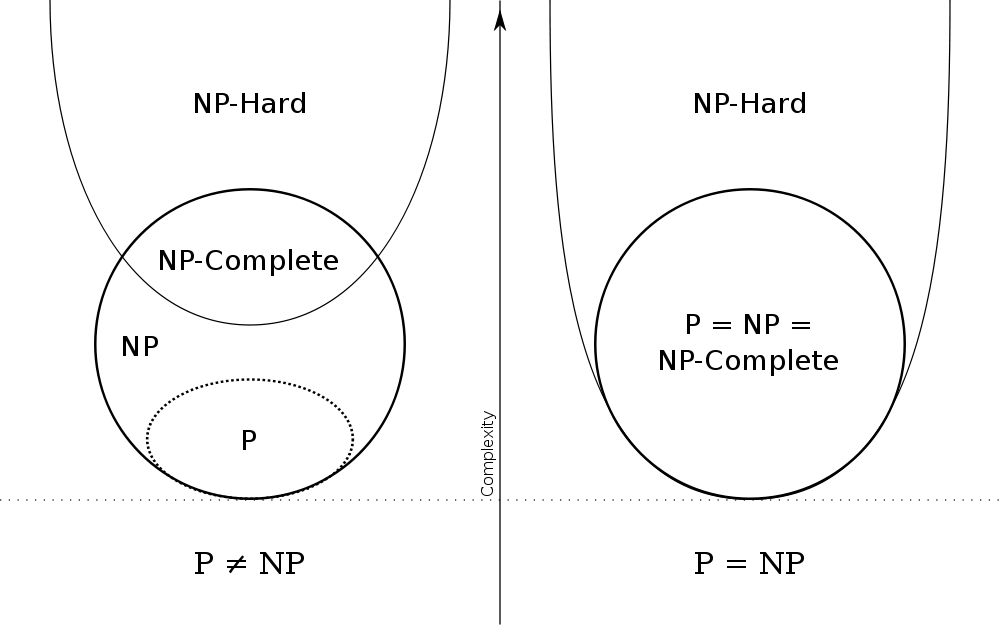
\includegraphics[width=1\textwidth, keepaspectratio]{imgs/np-complete.png}
\end{figure}
\noindent
It can be shown that every NP problem can be reduced to another, for example 3SAT. This is known as \textbf{Cook's theorem}. What makes NP-Complete problems important is that if a deterministic polynomial time algorithm can be found to solve one of them, every NP problem is solvable in polynomial time. 
\subsection{P, NP, or NP-Complete}
Let us once again go through the complexity classes so we can see if we have a problem $p$, is it in the class P, NP, or NP-Complete.

\subsubsection{P}
\begin{definition}
P is a complexity class that represents the set of all decision problems that can be solved in polynomial time. 
\end{definition}
\noindent
That is, given an instance of the problem, the answer yes or no can be decided in polynomial time. \textit{A full proof of whether a problem is in P requires an exhibition of a polynomial time algorithm.} Note that the algorithm can use other polynomial time algorithms as subroutines, called at most a polynomial number of times. Thus reductions from a polynomial problem. For example, given a connected graph $G$, can its vertices be coloured using two colours so that no edge is monochromatic?
\n
The algorithm to solve this problem can be done in polynomial time. We start with an arbitrary vertex and colour it red, then all of its neighbours blue and continue to another arbitrary uncoloured vertex. Stop when we run out of vertices or we are forced to make an edge have both of its endpoints be the same colour.
\subsubsection{NP}
\begin{definition}
NP is a complexity class that represents the set of all decision problems for which the instances where the answer is ``yes" or ``no" have proofs that can be verified in polynomial time.
\end{definition}
\noindent
This means that if someone gives us an instance of the problem and a certificate to the answer being yes, we can check the certificate is polynomial in size and is correct in polynomial time. For example integer factorisation is in NP. For large numbers in polynomial time, we cannot find its two factors, however, given the two factors, checking if they are correct is trivial. 
\subsubsection{NP-Complete}
\begin{definition}
NP-Complete is a complexity class which represents the set of all problems $A$ in NP, for which it is possible to reduce any other NP problem $B$ to $A$ in polynomial time. 
\end{definition}
\noindent
Intuitively, this means that we can solve $B$ quickly if we know how to solve $A$ quickly. More precisely, $B$ is reducible to $A$ if there exists a polynomial time algorithm $f$ which can transform instance of $B$ to instances of $A = f(B)$ in polynomial time. The answer to $B$ is yes is true if and only if the answer to $f(B)$ is true.
\n
To show that a problem is NP-Complete, we must show the problem is in NP and \textit{any problem} in NP can be transformed to it.

\subsubsection{Transformations}
Suppose there is a known NP-Complete problem \Pi. Then to show a new problem $p$ is NP-Complete, all we have to do it show that \Pi can be transformed to $p$. Now we just have to worry about one problem. 
\n
Because of this, it is really useful to have just \textbf{one} NP-Complete program that all other problems can reduce to. This was what Stephen Cook and Leonid Levin (independently) discovered after proving that SAT was NP-Complete. 

\subsection{Graph Colouring}
A graph colouring problem is a classical problem from map making. Maps can show regions more clearly if adjacent regions have different colours. The \textbf{4-Colouring Conjecture} is that any map can be coloured with 4 distinct colours. 
\n
This problem also has implications and importance in computers. Abstractly we can think of two adjacent nodes of some structured problem cannot be done together. This has importance in scheduling algorithms, as well as for example register-allocation for compilers. Two variables cannot be put into the same register if their value is used in the same part of the program. Graph colouring was shown to be \textbf{NP-Complete} by Karp.
\n

\subsection{Cook-Levin Theorem}
\begin{theorem}{\textbf{Cook-Levin Theorem}}
SAT is NP-Complete.
\end{theorem}
\noindent
The importance of Cook's theorem is that we now know \textit{if we have one NP-Complete problem, we can show several to be NP-Complete.} To show that SAT is NP-Complete we must first show that SAT is in NP, and then show that any other problem in NP can be reduced in polynomial time to a instance of SAT. In other words it requires showing
\begin{itemize}
\item If $p$ is a problem with an NP algorithm
\item ...then $p \leq SAT$
\end{itemize}
\begin{proof}
To show that SAT is in NP is easy. Simply non-deterministically guess an assignment to the variables, then we can check in polynomial time if each clause it true for that assignment. Now we have to prove for an arbitrary NP problem, that it can be reduced to SAT. 
\n
If we have an arbitrary problem $A \in \textsc{NP}$, this \textbf{implies:}
\begin{itemize}
\item We have a non-deterministic TM $M_{A}$ for $A$
\item For any word $w \in A$, $M_{A}$ on $w$ takes $p(|w|)$ time
\end{itemize}
We have to create a SAT instance that is satisfiable if and only if $M_{A}$ accepts $w$ in time $p(|w|)$. We have to ensure that the formula is polynomial in size. 
\end{proof}

\subsection{Why Polynomials?}
One question might be why we care so much about polynomials compared to the other complexity classes. Notice that both \textsc{P} and \textsc{NP} are an infinite union of polynomials. Each polynomial degree has more power than the next,
\begin{equation}
\textsc{DTIME}(n^{120}) \subset \textsc{DTIME}(n^{121})
\end{equation}
We know that many natural algorithms have polynomial time, such as merge sort and bubble sort. We also know that some natural algorithms are exponential and it is relatively clear that these exponential algorithms are much more expensive. 
\n
However, though it may seem that quadratic or even cubic time is much better than exponential, it is sometimes hard to reason that a degree one million polynomial ($n^{1000000}$) is much better than exponential. In the real world, not many algorithms with higher than the sixth power are known. In some cases such as linear programming, we prefer the worst case exponential algorithm compared to the worst case $n^5$ algorithm.
\n
Ultimately, polynomials is a class of algorithms with good theoretical properties and arguable good practical properties. Answers to the P = NP question also imply answers to separation of analogous deterministic vs non-deterministic questions.
\subsubsection{Extended Church-Turing Thesis}
The Church-Turing Thesis states that \textit{all reasonable models of computation have the same power in terms of recognising languages}. An extended version of the thesis is that \textit{all reasonable models of computation when restricted to polynomials have the same power}. This applies to all \textbf{deterministic} models and another way of stating it is any model can be simulated by any other model with at most polynomial slowdown. 
\n
We have seen that polynomially related changes involve:
\begin{itemize}
\item TM steps needed
\item Number of tapes
\item Number of states
\item Number of symbols needed
\end{itemize}
However, it is unknown whether it applies to non-deterministic computers and unknown whether it applies to quantum computers. Remember that this is just a \textbf{hypothesis} and cannot be proved, but can be disproved.

\section{Analysis of Algorithms}

\section{Analysing Recursive Programs}
Analysing algorithms is quite straightforward for iterative algorithms but more difficult for recursive algorithms. A key technical tool for this kind of analysis is \textbf{recurrence relations}. 
\begin{equation}
T(n)\ \text{is the time taken for input size}\ n
\end{equation}
A key insight is $T(n)T$ often depends of $T(m)$ for $m < n$. Such a relation is called a recurrence relation. For example the Fibonacci Recurrence can be defined as below:
\begin{equation}
F(n) = F(n - 1) + F(n+2)
\end{equation}
\begin{equation}
F(0) = 1,\ F(1) = 1
\end{equation}


\section{Reductions and Games}


\end{document}